\chapter{Vergleich entwickelter Rekonstruktions Algorithmus mit bereits vorhandenen (Matlab)}
\label{sec:rectification}

Die Rektifizierung, allem voraus vor allem die Optimierung des Rektifizierungvorgangs, von Stereo- oder auch mulitplen- Kamerasystemen, wird heutzutage von vielen Entwicklergruppen der Computer Vision untersucht(Der satz ist mist!). Es gibt mittlerweile viele Ansätze, jedoch funktionieren nicht alle bei den selben Fällen. So setzten zum Beispiel manche Rektifizerungsalgorithmen voraus, dass die Bilder von Kameras mit selber Auflösung aufgenommen wurden.

Der entwickelte Szenenrekonstruktionsalgorithmus wurde so entwickelt, dass eine Rektifizierung der Bilder, wie sie in vielen Programmen verwendet wird, nicht notwendig wird. Der Grund dafür ist, dass ein Algorithmus entsteht, welche auch mit Bildern unterschiedlicher Kameraauflösungen eine erfolgreiche Rekonstruktion vollbringt.\\

problem: kommt nicht mit anderen Kameraauflösungen zurecht. Zwei lösungen: einmal rekonstruktion über essentielle matrix oder neuer rektifizierungsalgorithmus.\\

Schreiben und erklären warum wurde ein Ansatzt ohne Rektifizierung in erwägung gezogen \\

sagen dass man erst einmal in den Workflow eines auf Rektifizierung basierten Programms aufzeigt\\



Eigener Ansatz implementierung eines Rektifizierungsalgorithmus zum test auf Funktionaliät unter schiedlicher Aflösungen \\

Ergebnisse Präsentieren\\

Ansatz Lösungen: Mein Ansatz rekonsturiert ohne dei ausgabebilder zu "kennen" und zu verändern, bbei rektifizierung wird mit den feriten Bildern gearbeitet, was bei unterschiedlichen Auflösungen zu starken verzerrungen kommen kann bei der Rektifizierung.

\section{Szenenrekonstruktion mit Rektifizierung}


Die Korrespondenzanalyse konnte um eine Dimension reduziert werden. Durch die
Rektifikation, die Generierung virtueller achsparalleler Stereosysteme, kann die Korrespondenzanalyse
zudem wesentlich einfacher implementiert werden. Korrepondierende
Bildpunkte liegen infolge der Rektifikation auf der gleichen Zeile beider Bilder.\cite{phdextrinsicPara}

Ein weiteres weit verbreitetes Verfahren, ist cor der Szenenrekonstruierung durch Triangulierung eine Rektifizierung beider Bilder vorzunehmen\cite{MatlabRec,ZZ,Javier,Fusiello}.\\ 

Da bestimmte Formen der Rektifizierung keine vorherige Kalibrierung der Kameras benötigen, wird diese Methode in den meisten gängigen Echtzeit-Szenenrekonstruktionen eingesetzt. \cite{Fusiello,Javier,R.H.}.\\



Definition einer Rektifizierung:
Rektifizierte Bilder müssen zwei Eigenschaften erfüllen. Zum einen müssen alle Epipolargeraden parallel zur x-Koordinatenachse verlaufen und zweitens müssen alle korrespondierenden Punkte die selben y-Koordinaten besitzen\cite{ZZ}.

 Die Grundidee hier hinter ist, dass die Kameramatrizen von zwei Kameras so aufgebaut sind dass die intrinsischen Parameter die selben sind, sie sich aber in ihren Rotationen und Translationen voneinander unterscheiden. Die extrinsischen Kameraparameter werden dann dementsprechend so manipuliert, dass die Bildebenen Achsenparallel zueinander stehen\cite{FusielloSite,Fusiello}. Um horizontale Epipolarlinien zu erhalten muss gleichzeitig die Basislinie zwischen den zwei Kamerazentren parallel zur neuen x-Achse beider Kameras sein. Zudem soll, um eine angemessene Rektifizierung zu gewährleisten, müssen konjugierende Punkte die selbe vertikale Koordinate haben. Dies wird hier durch die die Bedingung gewährleistet, dass beide Kameras die selben intrinsischen Parameter haben\cite{FusielloSite}.

\begin{minipage}{\linewidth}
	\centering
	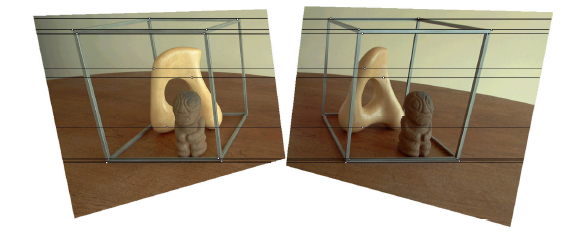
\includegraphics[width=.8\linewidth]{images/rectifiziertesBildAusZZ.png}
	\captionof{figure}{Beipiel eines rektifizierten Bildes. Quelle: \cite{ZZ}} 
\end{minipage}\\ \\


Hier erstmal schreiben warum genau, der Ansatz nicht mit unterschiedlichen Auflösungen läuft und auf den Workflow etwas genauer eingehen aber nicht übertreiben sonst fragen die da zu viel nach....


Mit Hilfe dieser Eigenschaften ist es somit möglich die enstandenen korresponierenden Epipolarlinien als horizontale Scanlinien zu benutzen\cite{Javier,ZZ}. Mit hilfe dieser Scanlinien und den darauf sich befindenden korrespondierenden Punkte ist es zum Beispiel Möglich eine Tiefenkarte des Bildes zu berechnen allein durch die Differenz der horizontalen Lage der korrespondierenden Punkte\cite{Javier,ZZ}. \\

\begin{minipage}{\linewidth}
	\centering
	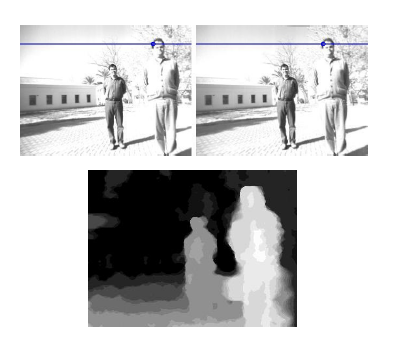
\includegraphics[width=.8\linewidth]{images/Disparity.png}
	\captionof{figure}{Beispiel einer einfachen Tiefenkarte eines Stereobildpaares nach der Rektifizierung. Quelle: \cite{Javier}} 
\end{minipage}\\ \\


Rektifizierung mit unterschiedlichen Aufnahme... warum funktioniert es in vielen Ansätzen nicht... was würde mit dem Bildpassieren? \\
Für Disparity maps müssen die horizontalen werte auf die selbe reihe passen. \cite{Javier,Fusiello}\\


standardvorgehen erklären\\

Beispielhafte implementierung einer Image recitfication anhand korrespondierender Punkte und der FUndamentalmatrix\\



Versuch unterschiedliche KAmeraauflösungen.. Bilder sind refkiifiziert aber Bild zwei ist komplett verzerrt... da Horizontale reiehn nicht übereinstimmen... 


Davor unbedingt erwähnen mit epipolen im undendlchen und so

\section{Rektifizierung mit Homographien}

In dieser Arbeit wurde ein Rektifizierungsalgorithmus nach \textit{Zhang}\cite{ZZ} implementiert. Diese recht aufwendige Art der Rektifikation zeichnet sich durch minimale Voraussetzungen an die Ursprungsbilder aus. Alle notwendigen Informationen zur Rektifikation werden aus der Fundamentalmatrix gewonnen. Zusätzlich zur Fundamentalmatrix muss noch die Lage der jeweiligen Epipole bekannt sein\cite{phdextrinsicPara}. Für die implementierte Rektifizierung wird pro Bild eine Homographiematrix $H$ und $H'$ aufgestellt. Die rektifizierung aller Bildpunkte $m_\sigma$ und $m'_{\sigma'}$ erfolgt durch Gleichung \ref{eq:rectifyPoints}

%Die Homographien $H$ und $H$ transformieren die Bildpunkte $m_\sigma$ und $m'_{\sigma'}$ zu rektifizierten Punkten $\bar{m}_\sigma$ und $\bar{m}'_{\sigma'}$

\begin{gather}
	\bar{m}_\sigma= H m_\sigma\\ \label{eq:rectifyPoints}
	\bar{m}'_{\sigma'}= H'm'_{\sigma'}
\end{gather}\\ 


Die Fundamentalmatrix, welche aus den Rektifizierten korrespondierenden Punkte resultiert, wird mit $\bar{F}$ bezeichnet\cite{ZZ,phdextrinsicPara}:


\begin{gather}
	\bar{m}'^T_{\sigma'}\bar{F}\bar{m}_\sigma = 0\\
	\leadsto m'^T_{\sigma'}H'^T\bar{F}Hm_\sigma=0\\	
	\leadsto F = H'^T[i]_\times H	
\end{gather}\\


Die Homographien $H$ und $H'$ werden in die projektiven Komponenten $H_p$ und $H_p'$ und die affinen Komponente $H_a$ und $H_a'$ unterteilt. Die affine Komponenten wird wiederum in zwei weitere Komponenten unterteilt. $H_r$ steht für eine Ähnlichkeitstransformation und $H_s$ bezeichnet eine Scherungstransformation\cite{ZZ,phdextrinsicPara}.


\begin{gather}
	H = H_a H_p  \;\;\;\; \leadsto	H = H_s H_r H_p \\
	H' = H_a'H_p'\;\;\;\; \leadsto 	H' = H_s'H_r' H_p'\\
\end{gather}


$H_p$ bezeichnet die projektive Komponenten und $H_a$ steht für die affine Komponente. Die affine Komponenten wird wiederum in zwei weitere Komponenten unterteilt. $H_r$ steht für eine Ähnlichkeitstransformation und $H_s$ beinhaltet einen Scherungstransformation. $H_p$ beinhaltet sämtliche projektiven Transformationen, welche dafür sorgen, dass der Epipol $e$ ins Unendliche projiziert wird und die Epipolarlinien parallel zueinander, jedoch noch nicht parallel zur horizontalen Achse sind\cite{ZZ,phdextrinsicPara}. $H_r$ ist eine Rotationsmatrix, welche die Epipolarlinien parallel zu horizontalen Achse ausrichtet. $H_s$ ist eine Scherungsmatrix, welche durch Minimierung versucht die durch die Rektifizierung entstandenen projektiven Verzerrungen bestmöglich auszugleichen\cite{ZZ,phdextrinsicPara}. \\
%Beim Prinzip der Rektifikation mittels Homographien wird eine projektive Abbildung zwischen zwei Ebenen verwendet\cite{phdextrinsicPara}. \\

Die Reihen der Homographiematrizen $H$ und $H$ beschreiben drei Linien $u, \, v$ und $w$, welche jeweils durch den Epipol verlaufen. Die Linien $v$ und $v'$ sowie $w$ und $w'$ sind korrespondierende Epipolarlinien. Durch diese geometrische Bedingung wird eine Verbindung der beiden Bilder zueinander. 
%Diese Bedingung schafft eine geometrische Verbindung beider Bilder zueinander und ist gerade bei der Minimierung der durch die Rektifizierung entstehenden Bildverzerrung von Bedeutung.

\begin{gather}
	H = \begin{bmatrix}
		u^T\\v^T\\w^T
	\end{bmatrix} =
	\begin{bmatrix}
		u_a&u_b&u_c\\
		v_a&v_b&v_c\\
		w_a&w_b&w_c
	\end{bmatrix}\\
	H' = \begin{bmatrix}
		u'^T\\v'^T\\w'^T
	\end{bmatrix} =
	\begin{bmatrix}
		u'_a&u'_b&u'_c\\
		v'_a&v'_b&v'_c\\
		w'_a&w'_b&w'_c
	\end{bmatrix}	
\end{gather}\\

Bevor die Matrizen $H$ und $H'$ in ihre projektiven und affinen Komponenten zerlegt werden, wird die letzte Komponenten $w_c$ und $w_c'$ durch Division eliminiert um somit skaleninvariante Matrizen $H$ und $H'$ zu bekommen\cite{ZZ,phdextrinsicPara}. 
%
%Für die Bestimmung der einzelnen Komponenten von $H$ und $H'$ werden diese in ihre projektiven und affinen Teilstücke zerlegt. Davor wird noch die letzte Komponente $w_c$ raus dividiert, um somit  skaleninvariante Matrizen $H$ und $H'$ zu bekommen. 

\begin{gather}
	H = \begin{bmatrix}
		u^T\\v^T\\w^T
	\end{bmatrix} =
	\begin{bmatrix}
		u_a&u_b&u_c\\
		v_a&v_b&v_c\\
		w_a&w_b&1
	\end{bmatrix}\\
	H' = \begin{bmatrix}
		u'^T\\v'^T\\w'^T
	\end{bmatrix} =
	\begin{bmatrix}
		u'_a&u'_b&u'_c\\
		v'_a&v'_b&v'_c\\
		w'_a&w'_b&1
	\end{bmatrix}	
\end{gather}\\


Die Matrizen $H_p$ und $H_p'$ beschreiben den projektiven Teil von $H$ und $H'$. Sie wirken sich sich auf den projektiven Teil eines Punktes aus und werden dazu verwendet die Epipole ins unendliche zu projizieren\cite{ZZ,phdextrinsicPara}.

%
%\begin{gather}
%	H = H_p \cdot H_a\\
%	H' = H'_p \cdot H'_a
%\end{gather}\\
%
%$H_p$ und $H_p$ beziehen sich nur auf die projektiven Komponenten ist die projektive Komponente, sie bezieht sich nur auf die letzte Zeile der Matrix $H$.  und wirkt sich somit auch nur auf die homogene Komponenten der mit ihr verrechneten Punkte aus. 

\begin{gather}
	H_p = 
	\begin{bmatrix}
		1&0&0\\
		0&1&0\\
		w_a&w_b&1
	\end{bmatrix}
\end{gather}\\

Für die affinen Komponeten $H_a$ und $H_a'$ gilt:

\begin{gather}
	H_a= H \cdot H^{-1}_p = 
	\begin{bmatrix}
		u_a-v_cw_b&v_cw_a-v_a&0\\
		v_a-v_cw_a&v_b-v_cw_b&v_c\\
		0&0&1
	\end{bmatrix}
\end{gather}
.

%Für die Matrizen $H_p'$ und $H_a'$ gilt das selbe. Die projektive Matrix sogt dafür, dass die Epipole beider Bilder ins unendliche gesetzt werden und die Epipolarlinien der Bilder jeweils parallel zueinander verlaufen. Zu Beginn wurde erwähnt dass es eine Zerlegung in eine projektive, eine Ähnlichkeits- und eine Scherungstransformation gibt. Die projektive Komponente ist mit $H_p$ und $H_p'$ bereits vollständig definiert. 

Des Weiteren gilt für $H_a$ und $H_a'$, dass jeweils nochmal in eine Rotationsmatrix $H_r$ und $H_r'$ und eine Scherungsmatrix $H_s$ und $H_s'$ zerlegt werden\cite{ZZ,phdextrinsicPara}.

%Was nun noch fehlt ist die Zerlegung der affinen Matrizen $H_a$ und $H_a'$ in ihre jeweiligen Ähnlichkeits- und Scherungstransformationen. 

\begin{gather}
	H_a = H_s \cdot H_r\\
	H_r = 
	\begin{bmatrix}
		v_b-v_cw_b&	v_a-v_cw_a&0\\
		v_a-v_cw_a&v_b-v_cw_b&v_c\\
		0&0&1
	\end{bmatrix}\\
	H_s = 
	\begin{bmatrix}
		u_a&u_b&u_c\\
		0&1&0\\
		0&0&1
	\end{bmatrix}
\end{gather}\\

%$H_r$ und auch $H_r'$ definieren eine Rotation und auch eine Verschiebung, welche die bereits parallelen Epipolarlinien beider Bilder zueinander parallel und horizontal ausrichtet. Durch die Verschiebung werden die korrespondierenden Epipolarlinien noch auf die selbe Höhe verschoben. Somit entstehen die gewünschten Scanlinien in den Bildern. Die Matrix $H_s$ und $H_s'$ wirken sich nur auf die $u$-Elemente der Matrix $H$ und $H'$ aus und definieren eine Scherung. Sie haben keine Auswirkung auf die Rektifizierung an sich aber sorgen dafür, dass die horizontale Verzerrung der beiden Bilder zueinander reduziert wird.\\

\subsection{Projektive Transformation}

Im Folgenden wird die Herleitung der Matrizen $H_p$ und $H_p'$ beschrieben. Die projektiven Matrizen $H_p$ und $H_p'$ werden von den Linien $w$ und $w'$ , welche durch den Epipol verlaufen bestimmt. $w$ und $w'$ sind nicht willkürlich. Definiert werden sie durch eine Richtung $z = \begin{bmatrix}
\lambda&\mu&0\end{bmatrix}^T$. $z$ soll dabei so gewählt werden, dass die durch die rektifizierung entstehenden Bildverzerrungen in beiden Bildern minimal bleibt. Die Linien $w$ und $w'$ werden wie folgt definiert.

%, welche die, durch die Rektifizierung entstehende, Bildverzerrung minimieren soll. Für beide Bilder werden $w$ und $w'$ folgendermaßen gewählt

\begin{gather}
	w = [e]_x \cdot z \label{eq:w}\\ 
	w'= F\cdot z \label{eq:w'}
\end{gather}\\


%(AB HIER WEITER SCHREIBEN)
%Jedes beliebige $z$ würde zwei korrespondierende Epipolarlinien definieren, um ein $z$ zu finden, welches die Verzerrung der Bilder minimiert, wird ein Kriterium aufgestellt, welches ein $z$ finden soll, dass die Verzerrung minimal halten wird. 
Unter der Minimierung versteht man in diesem Falle, dass versucht wird ein $z$ zu finden, welches $w = (w_a,w_b,w_c)^T$ und $w'=(w_a',w_b',w_c')^T$ so definiert, dass die Eintrage $w_a$ und $w_b$ und auch $w_a'$ und $w_b'$ in $H_p$ und $H_p'$ nahezu null sind. Anders ausgedrückt es wird versucht die projektive Matrizen $H_p$ und $H_p'$ so affin wie möglich zu machen\cite{ZZ}.\\ 

%Minimierung bedeutet in diesem Falle, dass versucht wird die Matrizen $H_p$ und $H_p'$ so affin wie möglich zu machen. So affin wie möglich bedeute, dass die Werte von $w_a$ und $w_b$ so nah wie möglich an den Wert 0 gebracht werden sollen.

\begin{gather}
	H_p = 	\begin{bmatrix}
		1&0&0\\
		0&0&1\\
		w_a&w_b&1
	\end{bmatrix}
\end{gather}

%Jedoch sollen sie nicht ganz null werden, da die projektive Matrix dann keine projektive mehr wäre, sondern eine affine.  Deswegen heißt es auch sie soll so affin wie möglich gemacht werden. Das selbe gilt natürlich auch für $w_a'$ und $w_b'$ aus $H_p'$. 

Sollte es der Fall sein, dass beispielsweise Epipole $e$ bereits im unendlichen wären, so wären $w_a = 0$ und $w_b = 0$. In diesem Fall wäre eine projektive Transformation für diesen Epipol nicht mehr nötig.\\

Für die Minimierung wird die Methode der kleinsten Quadrate auf angewandt. Die Methode der kleinsten Quadrate ist ein mathematisches Standardverfahren für eine Ausgleichsrechnung, mit deren Hilfe aus der Menge der Bildpunkten beider Bilder ein wert für $z$ ermittelt werden soll\cite{leastSquare}. Für $z$ gilt mit $z = \begin{bmatrix}\lambda&\mu&0\end{bmatrix}^T$ bereits die Bedingung, dass es sich um einen Punkt im unendlichen handeln soll. $\lambda$ und $\mu$, sollen dabei einen Wert annehmen, welcher am nächsten an den Punkteansammlungen beider Bilder ist. \\




%Es werden also die Gewichtungen der Punkte in beiden Bildern in der Methode der Anpassung der kleinsten Quadrate verbaut, welche versucht eine Funktion zu finden, die einen Wert für $z$ berechnen soll welcher die Bildverzerrung minimal hält. \textcolor{red}{Anders ausgedrückt man sucht einen Wert für $z$, welcher am nächsten an den gegebenen Punktesammlungen der jeweiligen Bildern dran liegt, wobei für $z$ bereits gilt, dass es sich um einen Punkt im Unendlichen handeln soll}\cite{ZZ,leastSquare}.

%
% Angenommenem, dass die Annäherungsfunktion $g(x)$ eine Funktion $f(x)$, mit $x \in [a,b]$, annähern soll, dann versucht die Methode, die Summe der Quadrate der oridnatischen Differenzen, welche zwischen den von der Funktion generierten Punkten und den Punkten aus den Daten gewonnen wird, zu minimieren\cite{leastSquare,Margulies.}. Zum Beispiel werden $n$ Datenpunkte angenommen, dann gilt:
%
%\begin{gather}
%	e = \sum_{i=1}^{n}[f(x_i)-g(x_i)]^2
%\end{gather}

Um ein solchen $z$ zu ermitteln, werden zunächst die Gewichtungen der Punkte beider Bilder benötigt. $p_i$ beinhaltet alle Punkte von Bild eins und $p_j$ beinhaltet alle Punkte von Bild zwei. Ein Punkt  $p_{i1} = \begin{bmatrix}p_{i1,u}&p_{i1,v}&1\end{bmatrix}^T$ aus Bild eins soll zu einem Punkt $p_{i1} = \begin{bmatrix}\frac{p_{i1,u}}{w_i}&\frac{p_{i1,v}}{w_i}&1\end{bmatrix}^T$ mit $w_i$ gleich der Gewichtung 

\begin{gather}
	w_i=w^Tp_i
\end{gather} 

transformiert werden. Dasselbe soll auch für die Punkte $p_j$ im zweiten Bild geschehen. Sind die Gewichtungen beider Bilder gleich, so ergibt sich keine projektive Verzerrung und sowohl $H_p$ also auch $H_p'$ sind in dem Fall affine Transformationen und die Epipole wären bereits im unendlichen. Angenommen beide Epipole befinden sich noch nicht im unendlichen, so können die Gewichtungen der Punkte beider Bilder nicht gleich sein\cite{ZZ}.\\

Das Ziel ist, die Abweichung der Gewichtungen der Punkte beider Bilder zueinander so gering wie möglich zu machen. Die Rektifizierung wurde anhand des synthetischen Beispiels in Kapitel \ref{sec:minimal} implementiert. Dem entsprechend bilden die Abbildungen der Eckpunkte des Quaders auf den Sensoren der virtuellen Kameras, die Punkte in $p_i$ und $p_j$ anhand welcher die Rektifizierung durchgeführt werden soll. \\

%Im Realbeispiel werden alle Pixel des Bildes verwendet. Die Rektifizierung wurde im aufgeführten Beispiel anhand des erstellten Minimalbeispiels durchgeführt, somit wurden die Eckpunkte des Quaders des jeweiligen Bildes für die das Minimierungskriterium verwendet.
%
% Es wird eine Funktion nach dem Prinzip der Anpassung der kleinsten Quadrate aufgestellt, welche die Abweichung der Gewichtung der Punkte in Bezug auf die Gewichtung des Bildzentrums $p_c$ berechnet.
 
Der Wert $p_c$ ergibt sich aus der Mittelung aller verwendeten Punkte eines Bildes $p_c = \frac{1}{n} \sum_{i=1}^{n} p_i$ und gibt den Bildmittelpunkt an. $w_c$ ist die Gewichtung am Bildmittelpunkt und wird berechnet mit

\begin{gather}
	w_c = w^Tp_c
\end{gather}


Die Abweichung der Gewichtungen wird bezüglich der Gewichtung des Bildzentrums $w_c$ gemessen. 

\begin{gather}
	\sum_{i-1}^{n}\Big[\frac{w_i-w_c}{w_c} \Big]^2\\
	\leadsto \sum_{i=1}^{n}\Big[\frac{w^T (p_i-p_c)}{w^Tp_c} \Big]^2
	\leadsto \sum_{i=1}^{n}\Big[\frac{w^T (p_i-p_c)(p_i-p_c)^Tw}{w^Tp_cp_c^Tw} \Big]
\end{gather}\\

%dessen Gewichtung ergibt sich aus $w_c= w^T p_c$. Die gesuchte Abweichung ausgedrückt in der Anpassung der kleinsten Quadreate ergibt dann die folgende Formel.\\
%
%\begin{gather}
%	\sum_{i-1}^{n}\Big[\frac{w_i-w_c}{w_c} \Big]^2\\
%	\leadsto \sum_{i=1}^{n}\Big[\frac{w^T (p_i-p_c)}{w^Tp_c} \Big]^2
%	\leadsto \sum_{i=1}^{n}\Big[\frac{w^T (p_i-p_c)(p_i-p_c)^Tw}{w^Tp_cp_c^Tw} \Big]
%\end{gather}\\

Vereinfacht lässt sich das auch in einer Matrixgleichung in Form von

\begin{gather}
	\frac{w^TPP^Tw}{w^Tp_cp_c^Tw} \label{eq:MinimizationBild1}
\end{gather}

angeben, in welcher für $P$ gilt:

\begin{gather}
	P=\begin{bmatrix}
		p_{1,u}-p_{c,u}&p_{2,u}-p_{c,u}&...&p_{i,u}-p_{c,u}\\
		p_{1,v}-p_{c,v}&p_{2,v}-p_{c,v}&...&p_{i,v}-p_{c,v}\\\label{eq:P}
		0&0&...&0	
	\end{bmatrix}
\end{gather}

Für die Punkte $p_j$ in Bild zwei ergibt sich dann entsprechend die Matrixgleichung:

\begin{gather}
	\frac{w'^TP'P'^Tw'}{w'^Tp_c'p_c'^Tw'}\label{eq:MinimizationBild2}
\end{gather} 


$w$ und $w^T$ werden nun noch mit ihren Definitionen aus den Gleichungen \ref{eq:w} und \ref{eq:w'} ersetzt und die Gleichungen \ref{eq:MinimizationBild1} und \ref{eq:MinimizationBild2} als Summiert und als eine Funktion von $z$ ausgedrückt\cite{ZZ}. 

%Gleichzeitig werden die Gleichungen \ref{eq:w} und \ref{eq:w'} summiert um die Gleichung zu erhalten, welche sich auf beide Bilder gleichzeitig bezieht und somit eine Lösung für $z$, das für beide Bilder gilt, gesucht werden kann.
%Das Ziel ist es einen Wert für $z$ zu finden, welches bis jetzt noch nicht ersichtlich in den Gleichungen vorkommt. Also werden
%Um einen Wert für $z$ zu finden, werden nun die Gleichungen \ref{eq:MinimizationBild1} und \ref{eq:MinimizationBild2} entsprechend minimiert.

\begin{gather}
	\frac{z^T[e]_x^TPP^T[e]_xz}{z^T[e]_x^Tp_cp_c^T[e]_xz}+\frac{z^TF^TP'P'^TFz}{z^TF^Tp_c'p_c'^TFz} \label{eq:funcZLong}
\end{gather}

Gleichung \ref{eq:funcZLong} wird noch vereinfach mit:

\begin{gather}
	A = [e]_x^TPP^T[e]_x\\
	B=[e]_x^Tp_cp_c^T[e]_x\\
	A'=F^TP'P'^TF\\
	B'= F^Tp_c'p_c'^TF\\
	\leadsto 
	\frac{z^TAz}{z^TBz}+\frac{z^TA'z}{z^TB'Fz}
\end{gather}
.

Da bereits fest gesetzt ist dass die dritte Kompontente von $z$ gleich 0 sein wird, wird $z$ im Folgenden als zweidimensionaler vektor mit $z = \begin{pmatrix}
\lambda\\ \mu\end{pmatrix}$ dargestellt. $A,B,A'$ und $B'$ sind 3x3-Matrizen, von denen dann nur noch der erste 2 $\times$ 2- Block wichtig ist.\\

Für eine nicht lineare Optimierung wird das gesamte Polynom aufgeteilt, so minimieren wir zunächst $\frac{z^TAz}{z^TBz}$ und danach $\frac{z^TA'z}{z^TB'z}$. So entstehen für $z$ zunächst zwei Lösungen $\hat{z_1}$ und $\hat{z_2}$, welche über eine Mittelung eine ersten Schätzung für $z$ geben\cite{ZZ}.

\begin{gather}
	z = \frac{\frac{\hat{z_1}}{\| z_1 \|}+\frac{\hat{z_2}}{\| z_2 \|}}{2}
\end{gather}\\

Da es sich um eine nicht lineare Optimierung handelt ist die Minimierung von  $\frac{z^TAz}{z^TBz}$ gleichzusetzen mit der Maximierung von  $\frac{z^TBz}{z^TAz}$. Beide werden als eine Funktion von $f(z)$ definiert. Matrix $A$ wird mit der Choleskyzerlegung\cite{FormelsammlungMatrizen} in zwei höhere Dreiecksmatrizen zerlegt $A = D^TD$. Dies geht nur da $A$ nachweislich eine symmetrische und positiv-definite Matrix ist\cite{Fortran77,FormelsammlungMatrizen}. Des Weiteren wird definiert, dass $y = Dz$ ist und $f(z)$ wird dann zu $\hat{f}(y)$\cite{ZZ}.

\begin{gather}
	A = D^TD\\
	y= Dz \leadsto z= D^{-1}y\\
	f(z)= \frac{z^TBz}{z^TAz}\\
	\leadsto 
	f(z)=\frac{z^TBz}{z^TD^TDz}\\
	\hat{f}(y)= \frac{y^TD^{-T}BD^{-1}y}{y^Ty}
\end{gather}

Da $y$ bis auf einen Skalierungsfaktor bestimmt ist, kann angenommen werden, dass $\parallel y \parallel = 1$ gilt. $\hat{f}(y)$ ist maximiert, wenn $y$ gleich dem Eigenvektor von $D^-TBD-1$ ist, welcher mit dem größten Eigenwert von $D^-TBD-1$ assoziiert wird\cite{ZZ}. Für $\hat{z_1}$ ergibt sich $\hat{z_1} = D^{-1}y$. Exakt das selbe Verfahren wird für die Bestimmung von $z_2$ mit  $\frac{z^TB'z}{z^TA'z}$ angewandt\cite{ZZ}.\\

%Zum Schluss erhalten wir dann einen Wert für $\hat{z_1}$ mit $\hat{z_1} = D^{-1}y$. Exakt das selbe Verfahren wird für die Findung von $z_2$ mit  $\frac{z^TB'z}{z^TA'z}$ angewandt.\\

Sind $z_1, z_2$ und durch Mittelung der beiden eine erste Schätzung für $z$ gefunden, so kann ein Wert für $z$ gesucht werden, welcher noch näher an ein optimales Ergebnis heranreicht. Beide Lösungen $z_1$ und $z_2$, werden in die Funktion $f(z)$ eingesetzt und es wird ein gemeinsames Minimum gesucht\cite{ZZ}. So kann iterativ eine optimale Lösung für $z$ gefunden werden. Ist der Wert für $z$ bestimmt, so kann dieser die Gleichungen \ref{eq:w} und \ref{eq:w'} eingesetzt werden und $w$ beziehungsweise $w'$ bestimmt werden. Die Einträge der Matrizen $H_p$ und $H_p'$ wären mit $w = (w_a,w_b,w_c)^T$ und $w' = (w_a',w_b',w_c')^T$ bestimmt\cite{ZZ}.\\

Auf diese Weise wurden im synthetischen Beispiel die Matrizen $H_p$ und $H_p'$ bestimmt und auf die Abbildungen des Quaders angewandt. Abbildung \ref{fig:RectOriginal} zeigt die unrektifizierten Abbildungen der Quader in den Kameras. In grün ist die Abbildung des Quaders in $C$ zu sehen und in rot ist die Abbildung des Quaders in $C'$. Abbildung \ref{fig:RectOriginalELines} zeigt in blau die Epipolarlinien beider Abbildungen, welche sich in den jeweiligen Epipolen treffen. 


%Abbildung 4.7 zeigt in rot den Quader des Minimalbeispiels wie er in Kamera zwei abgebildet ist und in grün wie er in Kamera eins abgebildet ist. Kamera zwei ist horizontal zu Kamera eins verschoben und um $45\circ$ zu Kamera eins um die eigene vertikale Achse ein gedreht. Die Auflösungen beider Kameras sind identisch, sprich die intrinsischen Kameraparameter sind die selben. Abbildung 4.8 zeigt die momentanen Epipolarlinien. Die Epipolarlinien von Bild eins, also dem grünen Abbild, sind bereits Parallel, was aber keine Voraussetzung für die Funktion des Rektifizierungsalgorithmus ist. Der Schnittpunkt der Epipolarlinien von Bild zwei, also dem Roten Abbild, treffen sich in einem Punkt und bilden somit den Epipol von Bild zwei. 

\begin{minipage}{\linewidth}
	\centering
	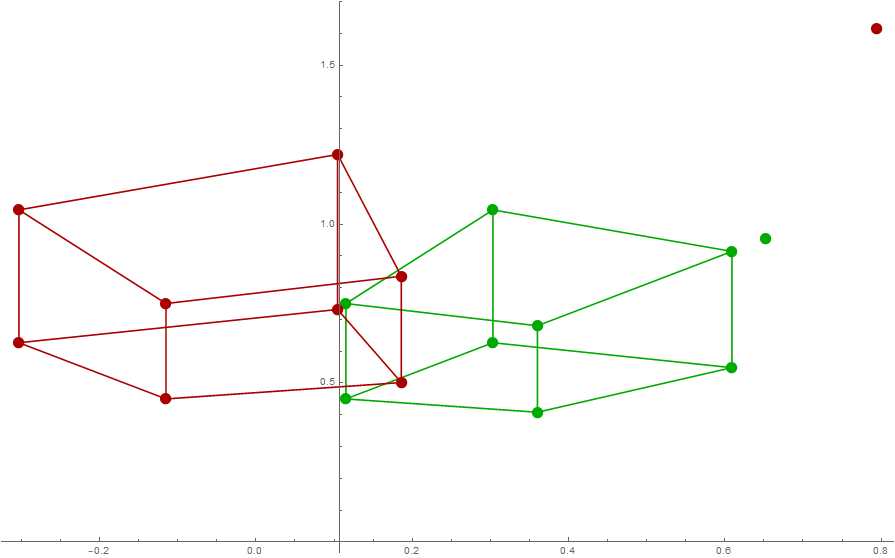
\includegraphics[width=.8\linewidth]{images/Rectification_one_same_Solutions.png}
	\captionof{figure}{Aufnahmen zweier Kameras mit den selben Auflösungen, Kamera eins(Grün) und Kamera(rot) zwei gelten jeweils \ensuremath{\zeta =1}}
	\label{fig:RectOriginal} 
\end{minipage}\\ 

\begin{minipage}{\linewidth}
	\centering
	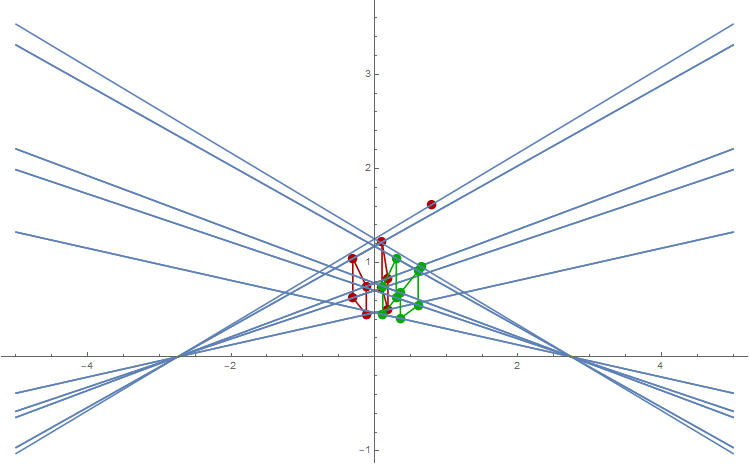
\includegraphics[width=.8\linewidth]{images/Rectification_two_same_Solutions.png}
	\captionof{figure}{Epipole für Kamera eins und Kamera zwei vor der Rektifizierung } 
	\label{fig:RectOriginalELines}
\end{minipage}\\


Nach Transformieren der Abbildungspunkte mit den Matrizen $H_p$ und $H_p'$ wurden die Epipole ins unendliche Transformiert. Die Epipolarlinien verlaufen jetzt parallel zueinander, jedoch noch nicht zwingend parallel zur horizontalen Achse. In Abbildung \ref{fig:RectSameHp} ist das Ergebnis der mit $H_p$ und $H_p'$ transformierten Bildpunkte zu sehen.

%Werden nun die Matritzen $H_p$ und $H_p'$ auf die jeweiligen Punkte der Bilder, $p_i$ für Bild eins und $p_j$ für Bild zwei, angewandt, so kann man eine erste Veränderung beobachten. Abbildung 4.9 zeigt beide Quader aus Abbildung 4.7 nachdem die jeweiligen Bildpunkte mit den projektiven Matrizen multipliziert wurden. Der Epipol in Bild eins bleibt natürlich wie zuvor im unendlichen, jedoch kann man erkennen, dass der rote Quader aus Bild zwei sich verändert hat. Sein Epipol wurde ins Unendliche transformiert und parallele Linien sind nun auch auf dem Bild parallel. Das die Epipolarlinien bereits horizontal parallel zur x-Achse verlaufen ist Zufall und ist nach der Anwendung der projektiven Matrizen auch noch nicht verlangt. Das Anpassen der Epipolarlinien, dazu gehört sie zunächst von beiden Bilder aus parallel zur x-Achse verlaufen zu lassen und dann noch sie so zueinander anzupassen, dass sie zu Scanlinien über beide Bilder verlaufen, verlgeiche Abbildung 4.12, folgt im nächsten Schritt. \\


\begin{minipage}{\linewidth}
	\centering
	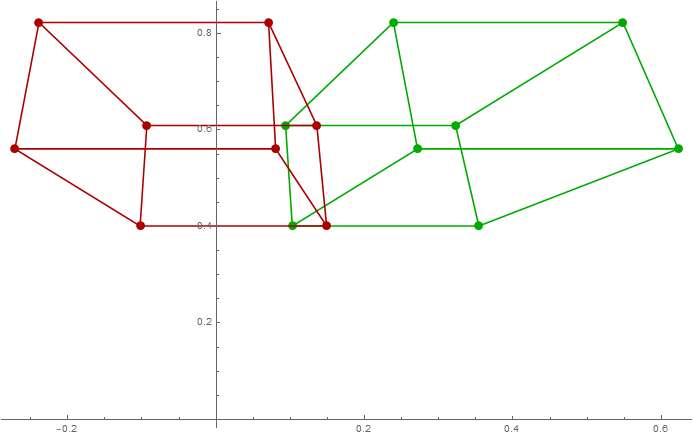
\includegraphics[width=1.\linewidth]{images/Rectification_Hp_same_Solutions.png}
	\captionof{figure}{Abbildung beider Bilder nach anwenden der Matrizen $H_p$ und $H_p'$. Die Epipole beider Bilder sind nun im unendlichen.} 
	\label{fig:RectSameHp}
\end{minipage}\\ \\

\subsection{Ähnlichkeitstransformation}

Nachdem die Epipole ins Unendliche verschoben wurden, müssen diese nun so rotiert und verschoben werden, dass die Epipolarlinien als Richtung $i = \begin{bmatrix}1&0&0\end{bmatrix}$ haben und die Epipolarlinien beider Bilder zu einheitlichen Scanlinien werden. Für die Ähnlichkeitstransformation wird davon ausgegangen, dass $w$ und $w'$ bereits bekannt sind.$H_r$ und $H_r'$ wurden bereits aus der Zerlegung von $H_a$ und $H_a'$ gewonnen.

\begin{gather}
	H_r = 
	\begin{bmatrix}
		v_b-v_cw_b&	v_a-v_cw_a&0\\
		v_a-v_cw_a&v_b-v_cw_b&v_c\\
		0&0&1
	\end{bmatrix}\\
	H_r' = 
	\begin{bmatrix}
		v_b'-v_c'w_b'&	v_a'-v_c'w_a'&0\\
		v_a'-v_c'w_a'&v_b'-v_c'w_b'&v_c'\\
		0&0&1
	\end{bmatrix}\\
\end{gather}

$w$ und $w'$ sind bereits bekannt, Mit Hilfe von $F$, können $v_a$ und $v_b$ ersetzt werden. Dazu kann die letzte Zeile von F nach $v_a, v_b$ und $v_c$ aufgelöst werden. Für $v_a', v_b'$ und $v_c'$ wird die letzte Spalte von F verwendet. So können folgende Gleichungen für $v_a, v_a',v_b, v_b', v_c$ und $v_c'$ gewonnen werden. 

\begin{gather}
	F = H'^T[i]_xH\\
	F=
	\begin{bmatrix}
		v_aw_a' - v_a'w_a&v_bw_a' - v_a'w_b&v_cw_a' - v_a'\\
		v_aw_b' - v_b'w_a&v_bw_b' - v_b'w_b&v_cw_b' - v_b'\\
		v_a - v_c'w_a&v_b - v_c'w_b&v_c-v_c'
	\end{bmatrix}\\
	v_a = F_{31}+v_c'w_a\\
	v_b = F_{32}+v_c'w_b\\
	v_c = F_{33}+v_c'\\
	v_a' = v_cw_a'-F_{13}\\
	v_b' = v_cw_b'-F_{23}\\
	v_c' = v_c -F_{33}
\end{gather}

Eingesetzt in die jeweiligen Matrizen $H_r$ und $H_r'$, entstehen die folgenden Matrizen in Gleichungen 4.114 und 4.115, welche nur noch die unbekannte $v_c'$ beinhalten. Die gemeinsame Variable $v_c'$ zeigt die geometrische Verbindung beider Bilder in ihrer Verschiebung entlang ihrer v-Richtung. Es wird also ein Offset von $F_33$ benötigt, um die Epipolarlinien horizontal zu Scanlinien auszurichten. \textcolor{red}{Den Wert für $v_c$ wird so ermittelt, dass das Minimum einer v-Koordinaten eines Pixel als minimum den Wert null besitzt }

\begin{gather}
	H_r = \begin{bmatrix}
		F_{32}-w_bF_{33}&w_aF_{33}-F_{31}&0\\
		F_{31}-w_aF_{33}&F_{32}-w_bF_{33}&F_{33}+v_c'\\
		0&0&1
	\end{bmatrix}\\
	H_r'=
	\begin{bmatrix}
		w_b'F_{33}-F_{23}&F_{13}-w_a'F_{33}&0\\
		w_a'F_{33}-F_{13}&w_b'F_{33}-F_{23}&v_c'\\
		0&0&1
	\end{bmatrix}
\end{gather}\\

Das Ergebnis der Bildpunkte $p_i$ und $p_j$ multipliziert mit den Matrizen $H_rH_p$ und $H_r'H_p'$ mit ist in Abbildung 4.10 zu sehen. Als letztes folgt noch die Scherungstransformation $H_s$ und $H_s'$ für die horizontale Entzerrung beider Bilder.\\ 

\begin{minipage}{\linewidth}
	\centering
	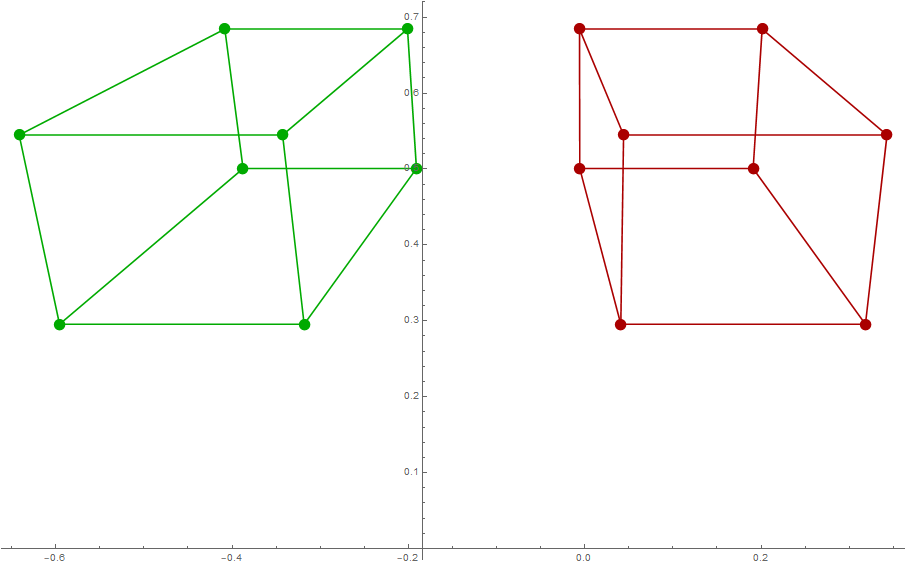
\includegraphics[width=1.\linewidth]{images/Rectification_HrHp_same_Solutions.png}
	\captionof{figure}{Abbildung beider Bilder nach anwenden der Matrizen $H_r \cdot H_p$ und $H_r' \cdot H_p'$. Die Epipolarlinien sind nun horizontal zueinander ausgerichtet} 
\end{minipage}\\ \\

\subsection{Scherungstransformation}

Die letzte Transformation, welche an den Bilder durchgeführt werden soll, ist die sogenannten Scherungstransformation. Sie soll vor allem dazu dienen, die horizontale Verzerrung der Bilder zueinander nochmal weiter zu minimieren. Die Matrizen $H_s$ und $H'_r$ wirken sich hauptsächlich auf die $u$ und $u'$ Komponenten aus. 

\begin{gather}
	H_s =\begin{bmatrix}
		u_a&u_b&0\\
		0&1&0\\
		0&0&1
	\end{bmatrix}\\
	H'_s =\begin{bmatrix}
		u'_a&u'_b&0\\
		0&1&0\\
		0&0&1
	\end{bmatrix}
\end{gather}

Um die richtigen Werte für $a, a', b$ und $b'$ zu bekommen, werden zunächst Punkte an den jeweiligen gegenüberliegenden Kanten der Bilder definiert. Da die Bilder des Quaders nicht aus tausenden von Pixeln bestehen, wie ein reales Bild, sondern nur über dessen Eckpunkte bestimmt ist, wird eine Bildbreite $w$ und $w'$ und eine Bildhöhe $h$ und $h'$ definiert. Die Höhen und Breiten der Bilder rahmen die abgebildeten Quader ein, somit wurde quasi eine Bildgröße für beide Bilder definiert. Nun können die Punkte an den Kantenhalbierenden $a = [\frac{w-1}{2} \; 0 \; 1]^T, b = [w-1 \; \frac{h-1}{2}\; 1]^T, c = [\frac{w-1}{2} \; h-1 \; 1]^T, d = [0 \; \frac{h-1}{2} \; 1]^T$ gebildet werden. Der Gedanke, der damit verfolgt wird ist, dass die Punkte der jeweiligen gegenüberliegenden Kanten mit einander verbunden werden können und dann so ausgerichtet werden sollen, dass sie sich wieder direkt gegenüber liegen. Schematisch wird as in Abbildung ???? aufgezeigt.

\begin{minipage}{\linewidth}
	\centering
	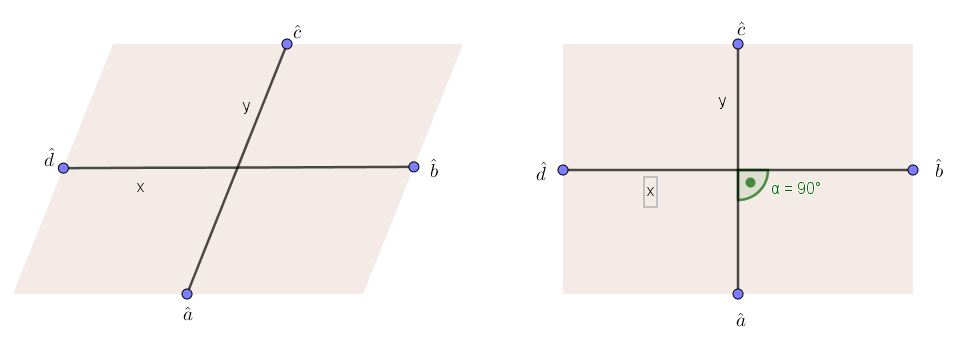
\includegraphics[width=.8\linewidth]{images/Scherungstransformation.png}
	\captionof{figure}{Die Abbildung verdeutlicht noch mal Schematisch, wie sich die Punkte ausrichten sollen. Bild a) zeigt die durch die Rektifizierung verschobenen Bildkantenmitten. Bild b= zeigt, wie sich die Bildkantenmitten durch die Scherungstransformation wieder ausrichten sollen.} 
\end{minipage}\\ \\

Die Punkte $a,b,c,d$ und auch $a',b',c',d'$ geben die Bildbreiten der noch unberührten Bilder an. Nach der Rektifizierung sind die Bilder so verzerrt, dass die Kanten mitten sich meistens nicht mehr direkt gegenüber von einander befinden. Die Punkte $a,b,c,d$ und $a',b',c',d'$ werden mit den Matrizen $H_p, H'_p, H_r$ und $H'_r$ verrechnet, so dass man die genaue neue Position der Kanten Mitten nach der Rektifizierung hat. 

\begin{gather*}
	\hat{a} = H_r\cdot H_p \cdot a\\
	\hat{b} = H_r\cdot H_p \cdot b\\
	\hat{c} = H_r\cdot H_p \cdot c\\
	\hat{d} = H_r\cdot H_p \cdot d\\
	\hat{a'} = H'_r\cdot H'_p \cdot a'\\
	\hat{b'} = H'_r\cdot H'_p \cdot b'\\
	\hat{c'} = H'_r\cdot H'_p \cdot c'\\
	\hat{d'} = H'_r\cdot H'_p \cdot d'\\
\end{gather*}

Um aus $\hat{a},\hat{b},\hat{c},\hat{d}$ und auch $\hat{a}',\hat{b}',\hat{c}',\hat{d}'$ wieder Punkte der affinen Ebene zu machen werden sie jeweils durch ihre dritte Komponenten geteilt, so das $\hat{a}_w,\hat{b}_w,\hat{c}_w,\hat{d}_w$ und $\hat{a}'_w,\hat{b}'_w,\hat{c}'_w,\hat{d}'_w$ jeweils den Wert eins besitzen. Danach können die Vektoren $\vec{x}$ und $\vec{y}$ aus den Differenzen der sich ursprünglich gegenüberliegenden Punkte gebildet werden.

\begin{gather}
	x = \hat{b}-\hat{d}\\
	y = \hat{c}-\hat{a}\\
	x' = \hat{b}'-\hat{d}'\\
	y' = \hat{c}'-\hat{a}'
\end{gather}

$x$ und $y$ sind Vektoren der euklidischen Bildebene. Die Rechwinkligkeit beider wird also erhalten, wenn gilt:

\begin{gather}
	(H_sx)^T(H_sy)= 0 \\
	(H'_sx')^T(H'_sy')= 0 
\end{gather}

Die Seitenverhältnisse der Bilder werden beibehalten, wenn gilt:

\begin{gather}
	\frac{(H_sx)^T(H_sx)}{(H_sy)^T(H_sy)} = \frac{w^2}{h^2}\\
	\frac{(H'_sx')^T(H'_sx')}{(H'_sy')^T(H'_sy')} = \frac{w'^2}{h'^2}	
\end{gather}

Für $u_a, u'_a, u_b$ und $u'_b$ jeweils Gleichungen auf Basis der jeweiligen Bild Höhen und Breiten $w,w',h,h'$ und $x,x',y$ und $y'$ und unter einhaltung der Aussagen der Gleichungen 5.118 bis 5.121, aufgestellt werden\cite{ZZ,ACM}. 

\begin{gather}
	u_a = \frac{h^2x_v^2+w^2+y_v^2}{hw(x_vy_u-x_uy_v)}\\
	u_b = \frac{h^2x_ux_v+w^2y_uy_v}{hw(x_uy_v-x_vy_u)}
\end{gather}

Selbe Gleichungen werden auch für $u'_a$ und $u'_b$ aufgestellt. Das Ergebnis der Scherungstransformation ist in Abbildung 5.17 dargestellt. \textcolor{red}{ Wie zu sehen ist, ist die Minimierung noch nicht zu hindert prozent perfekt, hierfür müsste man noch ein paar mehr Interationsschritte bei finden von $z$ einfügen.}(ICH WEIß GANZ EHRLICH NICHT WORAN ES LIEGT...)


\begin{minipage}{\linewidth}
	\centering
	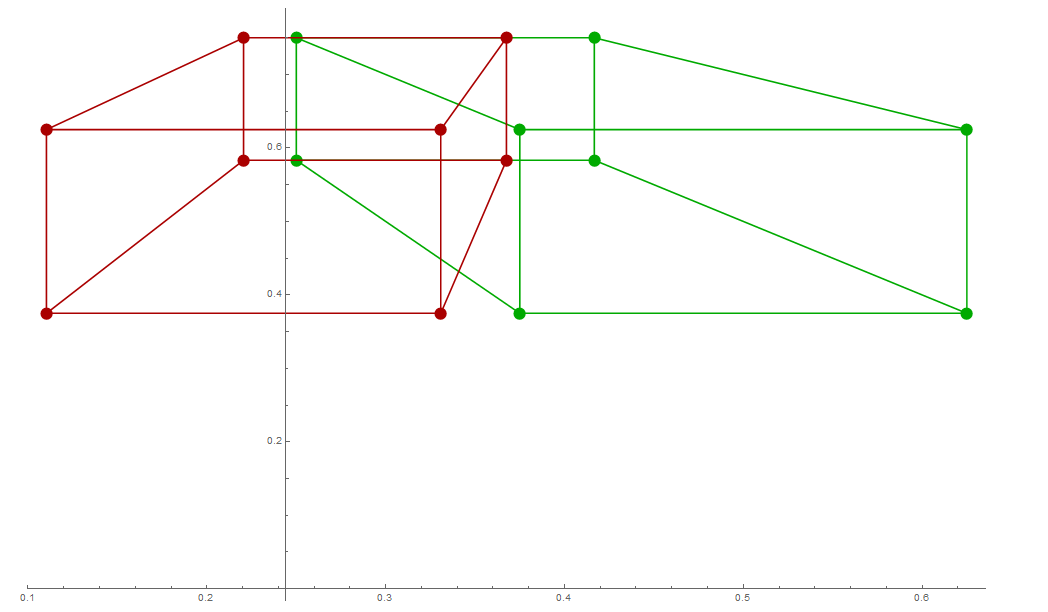
\includegraphics[width=1.\linewidth]{images/Rectification_HsHrHp_same_Solutions.png}
	\captionof{figure}{Abbildung beider Bilder nach anwenden der Matrizen $H_s \cdot H_r \cdot H_p$ und $H_s' \cdot H_r' \cdot H_p'$. Die horizontale Verzerrung wurde reduziert.} 
\end{minipage}\\ \\

\begin{minipage}{\linewidth}
	\centering
	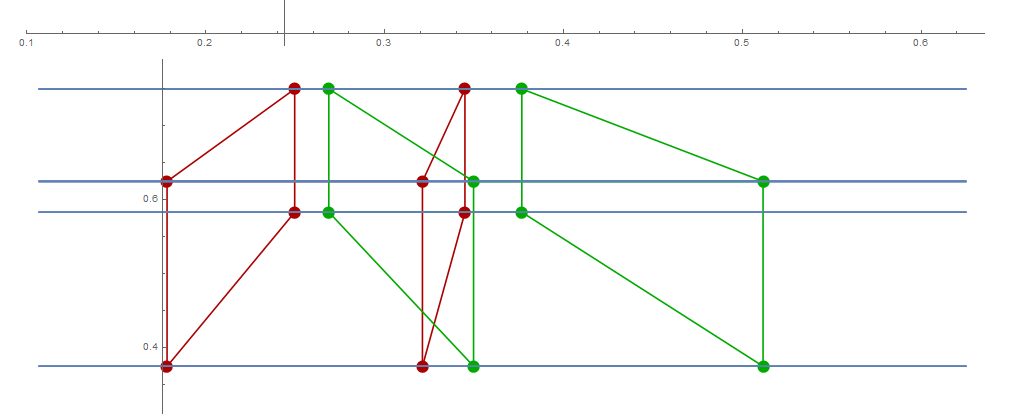
\includegraphics[width=1.\linewidth]{images/Rectification_four_same_Solutions.png}
	\captionof{figure}{In dieser Abbildung wurden die Epipolarlinien noch in den Grafikplot mit eingebaut} 
\end{minipage}\\ \\

\subsection{Rektifizierung mit unterschiedlichen Kamerauflösungen}

\begin{minipage}{\linewidth}
	\centering
	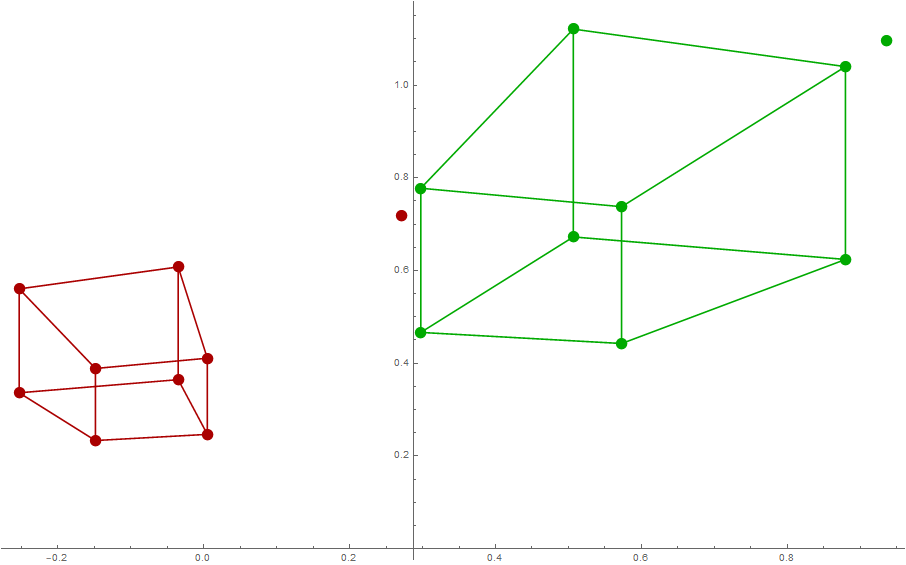
\includegraphics[width=1.\linewidth]{images/Rectification_one_different_Solutions.png}
	\captionof{figure}{Aufnahmen zweier Kameras mit unterschiedlichen auflösungen, Kamera eins(Grün) besitzt für \ensuremath{\zeta} den Wert 1 und für Kamera zwei(rot) gilt jeweils \ensuremath{\zeta_x = 1.2} und \ensuremath{\zeta_y = 3.1}} 
\end{minipage}\\ \\

(Normalerweise in realbildern wird das bild bei unterschiedlicher Auflösung nicht verzerrt sondern nur "Vergrößert" oder zurecht "geschnitten". Dadruch dass beide Quader in einem Koordinatensystem verbaut wurden sieht das so aus)


\begin{figure}[!htb]
	\minipage{0.48\textwidth}
	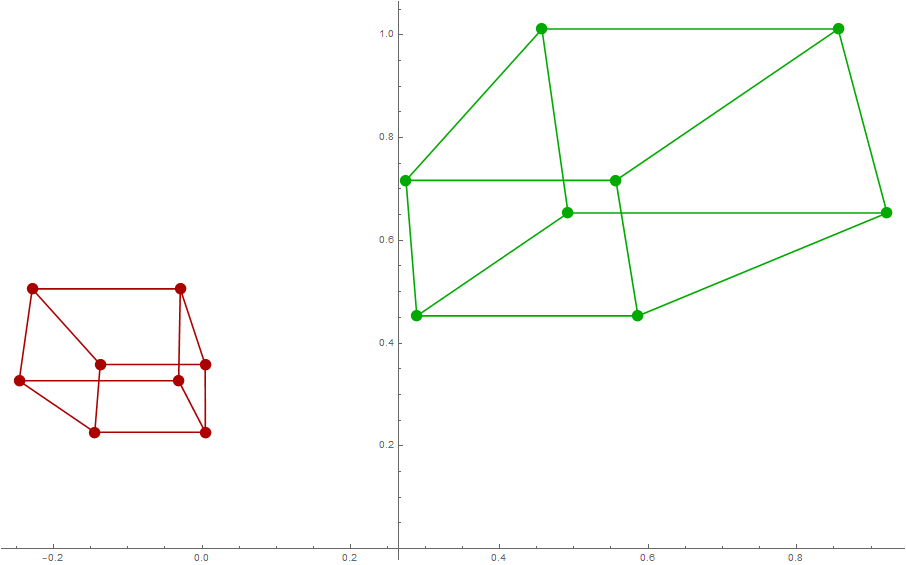
\includegraphics[width=\linewidth]{images/Rectification_Hp_different_Solutions.png}
	\caption{Epipole für Kamera eins und Kamera zwei vor der Rektifizierung}
	\endminipage\hfill
	\minipage{0.48\textwidth}
	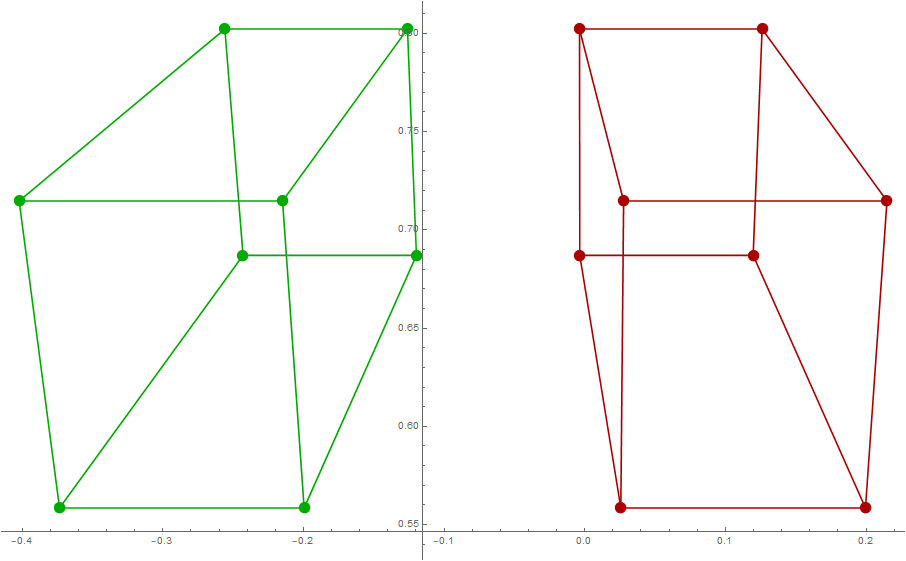
\includegraphics[width=\linewidth]{images/Rectification_HrHp_different_Solutions.png}
	\caption{Nach dem die drei Homographien auf die Punkte angewandt sind die Eckpunkte des Quaders auf beiden Bilder auf den selben corresüondierenden Epipolarlinien}
	\endminipage\hfill
	%\caption{Rekonstruierte Szene, wenn $K'$ mit einem Verhältnis von $[5:2]$ skaliert wurde}
	%\label{fig:RecT52}
\end{figure}

\begin{figure}[!htb]
	\minipage{0.48\textwidth}
	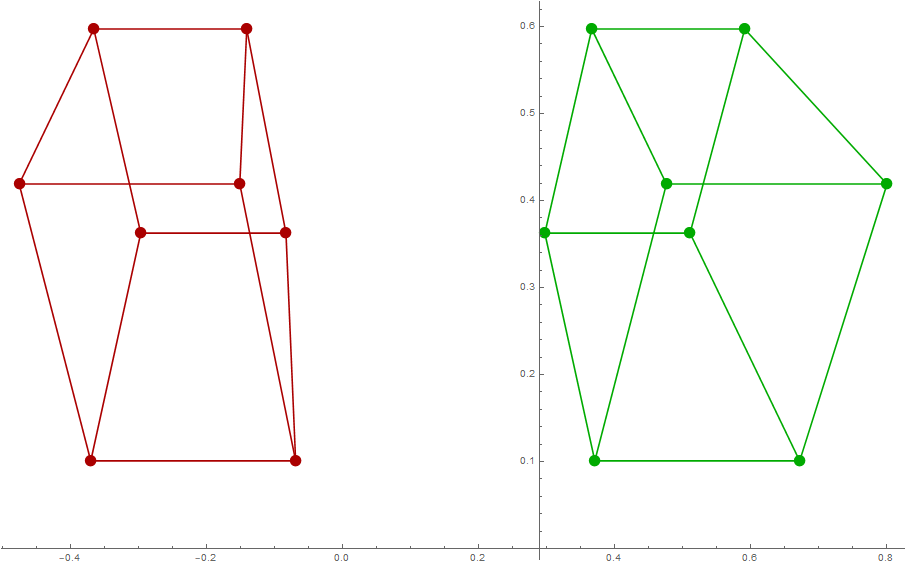
\includegraphics[width=\linewidth]{images/Rectification_HsHrHp_different_Solutions.png}
	\caption{In dieser Abbildung wurden die Epipolarlinien noch in den Grafikplot mit eingebaut}
		\endminipage\hfill
		\minipage{0.48\textwidth}
		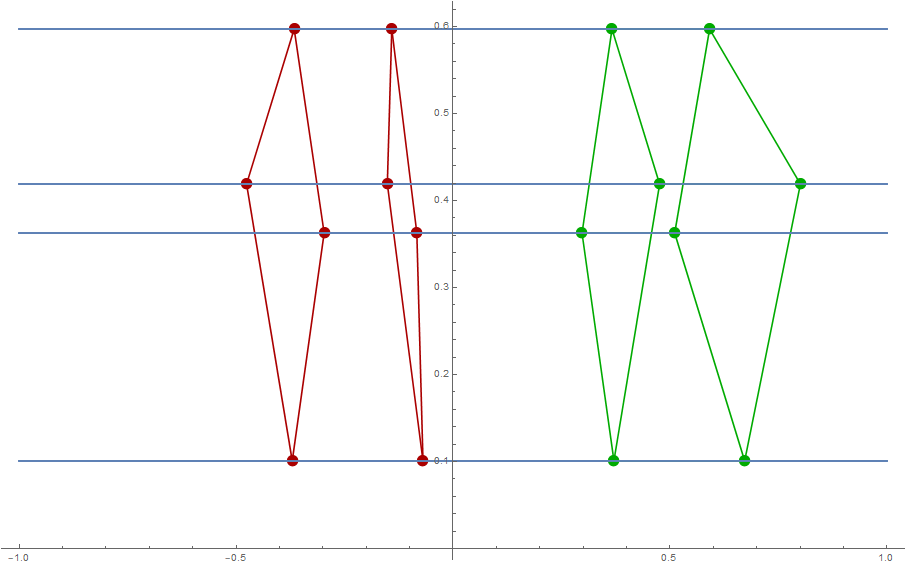
\includegraphics[width=\linewidth]{images/Rectification_four_different_Solutions.png}
		\caption{In dieser Abbildung wurden die Epipolarlinien noch in den Grafikplot mit eingebaut}
		\endminipage\hfill
		%\caption{Rekonstruierte Szene, wenn $K'$ mit einem Verhältnis von $[5:2]$ skaliert wurde}
		%\label{fig:RecT52}
\end{figure}

\pagebreak

Unterschiedliche Auflösungsverhältnisse führen wiederrum zu fehlern

\begin{figure}[!htb]
	\minipage{0.48\textwidth}
	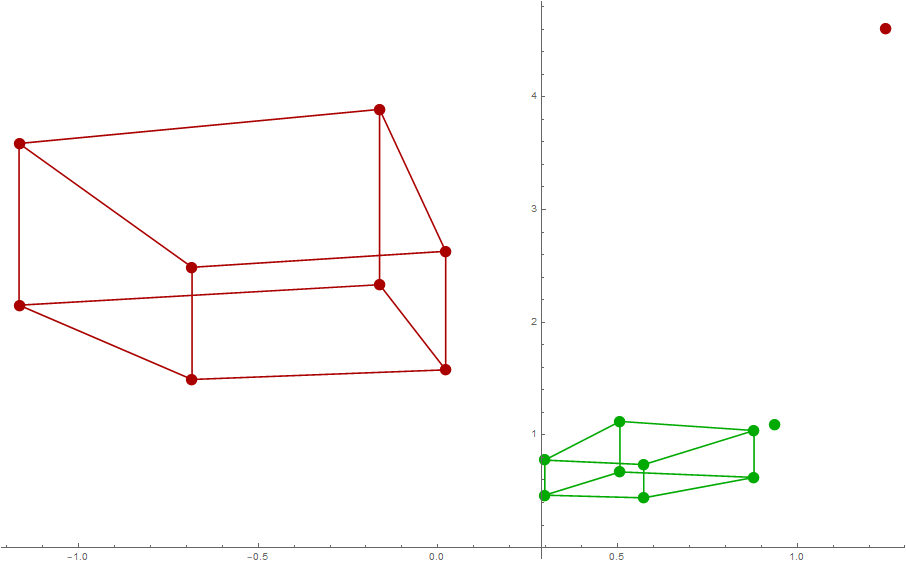
\includegraphics[width=\linewidth]{images/Rectification_Resolution_Abbild_verhaeltnisse.png}
	\caption{In dieser Abbildung wurden die Epipolarlinien noch in den Grafikplot mit eingebaut}
	\endminipage\hfill
	\minipage{0.48\textwidth}
	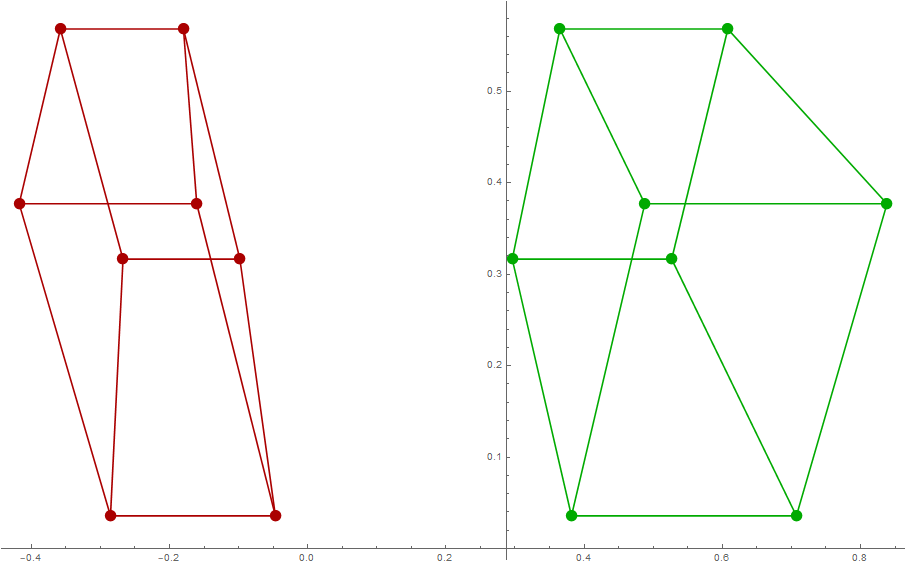
\includegraphics[width=\linewidth]{images/Rectification_Resolution_verhaeltnisse.png}
	\caption{In dieser Abbildung wurden die Epipolarlinien noch in den Grafikplot mit eingebaut}
	\endminipage\hfill
	%\caption{Rekonstruierte Szene, wenn $K'$ mit einem Verhältnis von $[5:2]$ skaliert wurde}
	%\label{fig:RecT52}
\end{figure}


%\begin{minipage}{\linewidth}
%	\centering
%	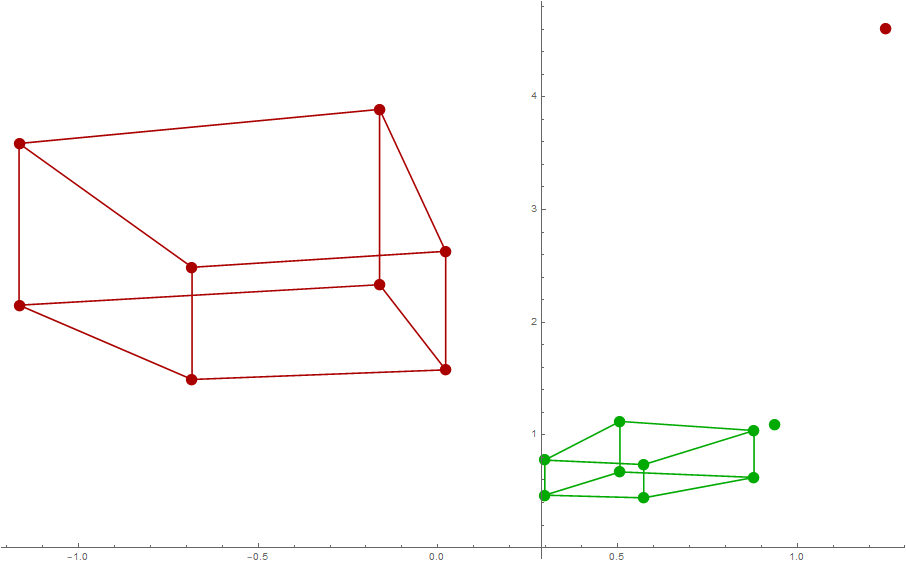
\includegraphics[width=1.\linewidth]{images/Rectification_Resolution_Abbild_verhaeltnisse.png}
%	\captionof{figure}{In dieser Abbildung wurden die Epipolarlinien noch in den Grafikplot mit eingebaut} 
%\end{minipage}\\ \\
%
%\begin{minipage}{\linewidth}
%	\centering
%	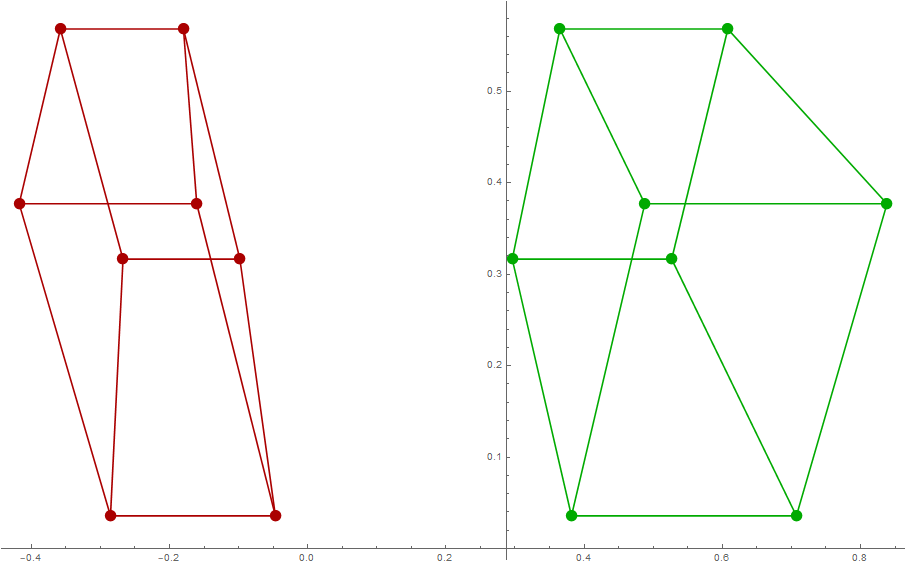
\includegraphics[width=1.\linewidth]{images/Rectification_Resolution_verhaeltnisse.png}
%	\captionof{figure}{In dieser Abbildung wurden die Epipolarlinien noch in den Grafikplot mit eingebaut} 
%\end{minipage}\\ \\



%Normalerweise wird die Welt als euklidischer 3D-Raum wahrgenommen. In manchen
%F¨allen jedoch ist es nicht anders m¨oglich oder gar w¨unschenswert,
%nicht die volle euklidische Struktur zu betrachten. Durch die Rektifizierung anhand von Homographien ist es erlaubt komplett im zweidimensionalen Raum zu arbeiten.
%
%
%, welche aus insgesamt drei unterschiedlichen Homographiematrizen sich zusammensetzt. 

%Zhangs Verfahren [Zha98] zus¨atzlich zur Lage des Epipols die Kenntnis der Fundamentalmatrix. \cite{phdextrinsicPara}\\
%
%%Diese recht aufwendige Art der Rektifikation zeichnet sich durch minimale Voraussetzungen
%%an die Ursprungsbilder aus. Alle notwendigen Informationen zur Rektifikation
%%werden aus der Fundamentalmatrix gewonnen\cite{phdextrinsicPara}\\
%
%Beim Prinzip der Rektifikation mittels Homographien wird eine projektive Abbildung zwischen zwei
%Ebenen verwendet. Die Zentralprojektion  selbst ist ebenfalls eine Homographie.\cite{ZZ,phdextrinsicPara}

%Die projektive Komponenten wird dabei in einem nichtlinearen Optimierungsprozess so affin wie möglich gemacht.\cite{Fusiello,ZZ,phdextrinsicPara}.\\




%Im folgenden wird zunächst der genaue Vorgang des implementierten Algorithmus genauer erklärt und 
%\textcolor{red}{des Weiteren werden zwei Beispiele vorgestellt, welche die Bilder des Minimalbeispiels einmal mit gleichen intrinsischen Parametern und einmal mit unterschiedlichen intrinsischen Parametern der Kamera aufzeigt. }. \\
%
%
%Die korrespondierenden Punkte werden mit $m_\sigma$ für das erste beziehungsweise $m'_{\sigma'}$ für das zweite Bild definiert, die Kamerazentren dementsprechend mit \textit{C} und \textit{C'}. \\
%
%%Bildebene der ersten Kamera wird mit \textit{I} definiert und die Bildebene von Kamera zwei mit \textit{I'}, die entsprechenden Epipole mit \textit{e} und \textit{e'}. \\
%
%
%Some previous techniques for finding image rectification homographies involve 3D constructions[1,
%4]. These methods find the 3D line of intersection between image planes and project the two images
%onto the a plane containing this line that is parallel to the line joining the optical centers.\\
%
%
%
%%
%%Diese Transformation wird durch eine Homographiematrix durchgeführt, welche sich aus den bereits erwähnten drei Komponenten zusammenstellt. 
%
%%Zu Beginn sei noch erwähnt dass wir pro Bild zwei unterschiedliche Homographien \ensuremath{H} und \ensuremath{H'} brauchen. \\
%
%Zu Begin wird die Beziehung aufgestellt, ein dass ein Korrespondierendes Punktepaar $m_\tau$ und $m'_{\tau'}$
%
%Für einen rektifizierten Punkt $\bar{m}_\sigma$ und $\bar{m}'_{\sigma'}$ soll gelten, dass
%
%\begin{gather}
%	\bar{m}_\sigma= H m_\sigma\\
%	\bar{m}'_{\sigma'}= H'm'_{\sigma'}
%\end{gather}\\
%
%Die Fundamentalmatrix, welche aus durch die Rektifizierten korrespondierenden Punkte resultiert, wird mit $\bar{F}$ bezeichnet\cite{ZZ,phdextrinsicPara}:
%
%
%\begin{gather}
%	\bar{m}'^T_{\sigma'}\bar{F}\bar{m}_\sigma = 0\\
%	\leadsto m'^T_{\sigma'}H'^T\bar{F}Hm_\sigma=0\\	
%	\leadsto F = H'^T[i]_\times H	
%\end{gather}\\
%
%Ziel ist es den Epipol ins Unendliche zu verschieben, um
%zu einer parallelen Anordnung der Epipolarlinien zu gelangen. Durch eine ¨Uberf¨uhrung
%der projektiven Geometrie in den affinen Raum soll ¨uber die Homographiematrizen
%eine Rektifikation der Bilder durchgef¨uhrt werden\cite{ZZ,phdextrinsicPara}.
%
%Das Ziel ist es diese zwei Homographien in deren bereits erwähnten projektiven und affinen Komponenten zu zersetzten, wobei diese die jeweils entstehenden Bildverzerrungen minimieren sollen.